\documentclass[times, utf8, seminar, english]{fer}
\usepackage{booktabs}
\usepackage{epigraph}
\usepackage{mathtools, amsmath,amsfonts,amssymb, amsthm}
\usepackage{hyperref}
\usepackage{fancybox}
\usepackage{graphicx}
\graphicspath{ {img/} }
\usepackage{etoolbox}

\makeatletter
\patchcmd{\chapter}{\if@openright\cleardoublepage\else\clearpage\fi}{}{}{}
\makeatother
\usepackage{minted}
\begin{document}
\theoremstyle{definition}
\newtheorem{definition}{Definition}[section]
\title{iproute2 and iptables packet}
\author{Neven Miculini\'{c}}

\maketitle
\tableofcontents

% Sadrži li seminar sve od navedenog: uvod, sadržaj, zaključak, popis literature? [yes]
% Sadrži li tekst seminara pravopisne pogreške? [TODO]
% Je li tekst seminara jasan i koherentan odnosno sadrži li sve potrebne informacije za razumijevanje? [TODO]
% Jesu li margine teksta u seminaru poravnate (justified)? [yes]
% Jesu li tvrdnje u tekstu seminara jasne i argumentirane? [yes, TODO]
% Jesu li sve slike i tablice referencirane (navedene) u tekstu seminara prije nego što se pojavljuju?
% Jesu li sve slike u seminaru čiste i bez pikselizacije ili razmazivanja? [yes]
% Postoje li tablice u seminaru pohranjene kao slike? (Ako su pohranjene kao slike, tada u pdf dokumentu sa seminarom ne možete mišem označiti odgovarajući tekst). [no]
% Sadrži li tekst seminara neki od neprimjerenih ili nepreciznih izraza uključujući: napretkom čovječanstva, znate ono kad, recimo da, konekcija, mejl, vrti se ili izravno obraćanje čitatelju (vi ste vjerojatno mislili), izražavanje u prvom licu jednine (sada ću objasniti) ili množine (problem koji često imamo)? [no, TODO]
% Koliko vam se čini da je bilo složeno pronaći istinite informacije, obraditi temu te ju prikazati? [medium hard]
% Ukupna ocjena za oblikovanje tekstualnog dijela seminara?
% Kakav opći dojam na vas ostavlja seminar (pdf dokument)? Biste li ga rado opet čitali. Biste li ga s ponosom pokazivali drugima? Biste li ga koristili u neki svojim drugim predavanjima ako je prikladan?
% Ima li video seminara uvod/uvodnu špicu pripremljenom u skladu s uputama?
% Je li siljed izlaganja u videu seminara smislen i razumljiv?
% Ocijenite kvalitetu slike videa.
% Ocijenite kvalitetu zvuka (naracije) videa.
% Kakav opći dojam na vas ostavlja video materijal? Biste li ga rado opet gledali. Biste li ga s ponosom pokazivali drugima? Biste li ga koristili u neki svojim drugim predavanjima ako je prikladan?

\chapter{Introduction}

Networking is one of the most important topic in the everyday computer use. Almost every meaningful action we do in digital world, sooner or later involves networkings. Whether it's simply performing backups, viewing facebook messages, sending emails, or accessing databases and utilizing VPN/SSH.

As in any complex system, networking included, many things may go haywire and multiple attacks are possible. China accidently routed 15\% of internet trafic in April 2010~\cite{HowChina98:online}. Viruses are spread through the network. The huge throughput makes it hard and challenging problem to tame, understand and navigate.

For the computer forensics purpose, this seminar describes bacis linux networking primities, from the time network packet enters the machine, reaches local process, and exits the machine.

It describes two tools consisting used most commonly in Linux networking. First is iptables, part of Netfilter project. Netfilter~\cite{netfilte6:online} is a framework providing various kernel hooks within network stack allowing user to modify and alter network packages. IPtables is their most commonly used utility. It shall be decribed in more detail in the chapter~\ref{chp:iptables}.

Iproute2~\cite{shemming47:online} is a collection of userspace utilities for controlling and monitoring various aspects of networking in the Linux kernel, including routing, network interfaces, tunnels, traffic control, and network-related device drivers. In this seminar the focus in only on the routing, and just a brief introduction and basic/most common commands.

\chapter{iptables}
\label{chp:iptables}
This chapter describes packet path through various iptables tables and chains. The rest of the chapter is dedicated for explaining basic ip tables concept
Visual overview can be seen in figure~\ref{fig:iptables_traverse}. This chapter is introducion in the iptables concept. For more information about syntax refer the manual page \verb|man iptables|.

\begin{figure}
    \centering
    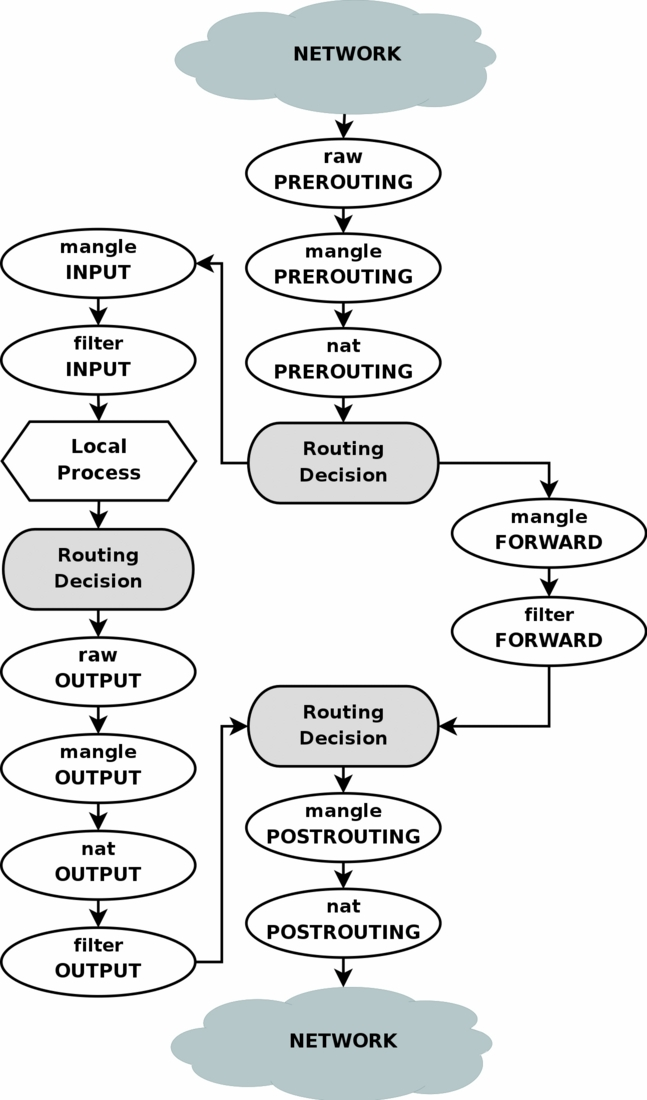
\includegraphics[width=0.8\textwidth]{tables_traverse}
    \caption{Overview of iptables. The lowercase word on top is the table and the upper case word below is the chain. Source~\cite{Iptables99:online}}
    \label{fig:iptables_traverse}
\end{figure}

\section{Rule}
    The most basic construct is an if-then rule. It's if side can be matched on various attributes -- packet's interface, protocol, source and destination IP adress, or even custom BPF~\cite{BPFthefo6:online} can be used. Upon rule matching, their 'then' side is executed, called \emph{target} within this context.

    The most common rule targets are ACCEPT, DROP, REJECT ones which perform packet filtering. In NAT table, common ones are DNAT, SNAT and MASQUERADE which perform IP:port NATing. NAT related targets are explained in section~\ref{sec:NAT}. Other common rule targets are LOG and jump to another chain. Chain jumping is further explaing in section~\ref{sec:chain}.

\section{Chain}
\label{sec:chain}
    Chain is a list of rules which are matched in order. Rule can be terminal (most of them) or nonterminal (e.g. LOG,  ULOG). Upon reaching the terminal rule (e.g. DROP) chain has reached its end. Chain can have it's default policy (e.g. DROP for table filter in INPUT chain).
    There are two types of chains -- system (PREROURING, INPUT, FORWARD, OUTPUT, POSTROUTING) and user defined chains.
    User defined chains target jump within the same table (e.g. jump to user defined chain).
    They are created with \verb|iptables -N <chain_name> -t <table name [filter default]>|.
    Chain traversal is depicted in figure~\ref{fig:iptables_subtraverse}. System chains are:

    \begin{itemize}
        \item PREROURING -- Packet arriving in the kernel before any routing
        \item INPUT -- Packet is destined for the local process
        \item FORWARD -- Packet isn't destined for the local process
        \item OUTPUT -- Packet originated from local process
        \item POSTROUTING -- Packet departing from the machine after all routing takes place
    \end{itemize}
    Refer to figure~\ref{fig:iptables_traverse} for their interaction.

    \begin{figure}
        \centering
        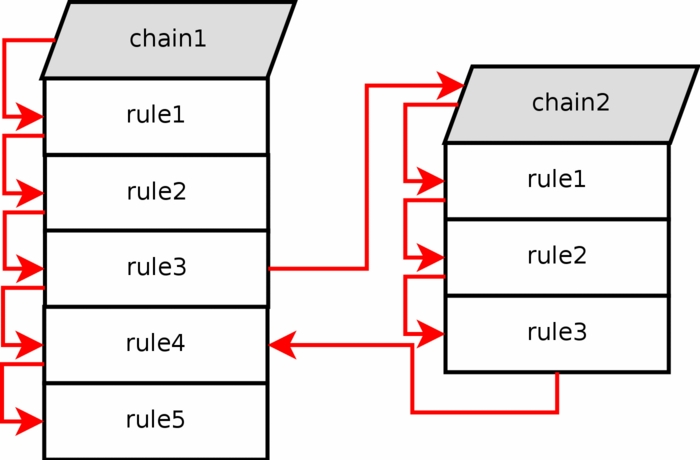
\includegraphics[width=0.8\textwidth]{table_subtraverse}
        \caption{Table chain subtraverstion. Source~\cite{Iptables99:online}}
        \label{fig:iptables_subtraverse}
    \end{figure}
\section{Tables}
    Tables are bread and butter of this package. Each table defines specific hooks in the kernel for various system chains. Each table is composed of multipe chains, what system defined ones, what user defined chains.
    There are 5 tables:
    \begin{itemize}
        \item raw -- applied before any connection tracking takes place. Used mostly to disable connection tracking since it's moderatly expensive. More information about connection tracking in subsection~\ref{subsec:conn-track}
        \item mangle -- Mostly used for quality-of-service (QoS) header bit setting.
        \item filter -- packet filtering (DROP, ACCEPT and REJECT tagets)
        \item nat -- NATing packages (DNAT, SNAT, MASQUERADE)
        \item security -- packet marking (SECMARK, CONNSECMARK) for SELinux. They are out of scope for this seminar.
    \end{itemize}
    Refer to link~\cite{Iptables27:online} for more detail. To view all chains and rule in particular table use \verb|iptables -vnL -t <table_name>|.

\section{Extensions}
    Iptables offers multiple modules you can use. They extend the basic functionality.
    You can view all installed modules by \texttt{ls -l /lib/iptables} and iptables will load all required modules dynamically. One of the most common ones is connection tracking. For other refer to their manual pages and documentation.

    \subsection{Conection tracking}
    \label{subsec:conn-track}
    If connection tracking is enabled (and can be disabled in raw TABLE with \texttt{-j NOTRACK} for rule match) each packet can be in following states:
    \begin{itemize}
        \item NEW -- first packet of the connection
        \item ESTABLISHED -- both server and client have sent a package
        \item RELATED -- related connection to an enstablished one. Protocol specific (e.g. there's FTP, IRC, etc. support in the kernel for RELATED connection tracking)
        \item INVALID -- connection state cannot be determined
    \end{itemize}

\chapter{IPtable examples}

\section{NAT}
\label{sec:NAT}

For NAT there are three specific targets related to NATing:
\begin{itemize}
    \item SNAT -- Source Network Address Translation. Exit packets source IP and port are rewriten to supplied source IP address. It is only valid in nat table within POSTROUTING chain. Downside is our source IP address must be known and static (or static range). Examples:
    \begin{minted}{bash}
# Change source addresses to 1.2.3.4.
iptables -t nat -A POSTROUTING -o eth0 -j SNAT --to 1.2.3.4

# Change source addresses to 1.2.3.4, 1.2.3.5 or 1.2.3.6
iptables -t nat -A POSTROUTING -o eth0 -j SNAT \
    --to 1.2.3.4-1.2.3.6

# Change source addresses to 1.2.3.4, ports 1-1023
iptables -t nat -A POSTROUTING -p tcp -o eth0 -j SNAT \
    --to 1.2.3.4:1-1023
    \end{minted}
    \item DNAT -- Destination Network Address Translation. It changes the package reciepeing, useful for servers behind firewall. It is only valid within nat table and PREROURING and OUTPUT chain. Examples:
    \begin{minted}{bash}
iptables -t nat -A PREROUTING -p tcp -d 15.45.23.67 --dport 80 \
    -j DNAT --to-destination 192.168.1.1-192.168.1.10
    \end{minted}
    \item REDIRECT -- DNAT but make destination local host. Only the port is changed.
    \begin{minted}{bash}
iptables -t nat -A PREROURING -p tcp -o eth0 -j REDIRECT \
    --to-ports 1234
    \end{minted}
    \item MASQUERADE -- it's similar to SNAT, but it doesn't require source IP address. It automatically grabs IP address information from sending interface. This is used in dymanically assigned IP connections. Example:
    \begin{minted}{bash}
iptables -t nat -A POSTROUTING -p TCP -j MASQUERADE
    \end{minted}
    I've used in real life while configuring OpenVPN server on google cloud, since google cloud instances only allow outgoing trafic with the source IP equals intance IP.
\end{itemize}

\section{Disabling internet access for specific device at specific time}

For example you might have a really smart teen adicted to the internet.
And you'd like disabling his internet access at the router level at certain times, while keeping rest functioning.
It can be simly done with one iptables command and few extra modules

\begin{minted}{bash}
iptables -A PREROURING -m mac --mac-source 00:0F:EA:91:04:08 \
    -m time --timestart 9:00 --timestop 18:00 -j ACCEPT
iptables -A PREROURING -m mac --mac-source 00:0F:EA:91:04:08 \
    -j DROP
\end{minted}

This is more efficient than IP filtering since you're probably running DHCP on your network dynamically assigning IP addresses.
Nevertheless, it's easy for attacker (your teen) to figure out his MAC address is filterer, and to spoof it.
Yet, hopefully by the time he figures it out, he'll already be a functional adult.


\chapter{Routing tables}
iproute2~\ref{shemming47:online} is the moden Linux networking toolkit. It's installed by default on almost all Linux distributions, or available from package manager. This explains only the basic routing primitives and usages. For more details refer to the man page, or this cheetcheet~\cite{iproute285:online}. All IP subnet examples shall use CIDR~\cite{Classles63:online} notation. Also a brief remined about two network stack models. OSI:
    \begin{itemize}
        \item layer 7 -- application layer
        \item layer 6 -- presentation layer
        \item layer 5 -- session layer
        \item layer 4 -- transport layer (e.g. UDP, TCP)
        \item layer 3 -- network layer (e.g. IP, ICMP, IPSec)
        \item layer 2 -- data link layer (e.g. ARP, IEEE 802.3)
        \item layer 1 -- physical layer (e.g. Bluetooth, IEEE 802.3, IEEE 802.11)
    \end{itemize}
    and internet protocol suite:
    \begin{itemize}
        \item Application layer (e.g. HTTP, DNS, IMAP)
        \item Transport layer (e.g. TCP, UDP)
        \item Internet layer (e.g. IP)
        \item Link layer (e.g. PPP, IEEE 802.11)
    \end{itemize}

First basic comand is \verb|ip route| which display current routes. On my computer the following is the display:
\begin{verbatim}
default via 192.168.121.1 dev wlp1s0 proto dhcp metric 600
172.17.0.0/16 dev docker0 proto kernel scope
    link src 172.17.0.1
172.18.0.0/16 dev br-8fd3cee01eeb proto kernel scope
    link src 172.18.0.1 linkdown
192.168.121.0/24 dev wlp1s0 proto kernel scope link
    src 192.168.121.194 metric 600
\end{verbatim}
In the first colum are the destination addresses for which this rule matches. For matching the longest matching prefix is used --> that mean if we have two rules:
\begin{verbatim}
172.17.0.0/16 dev eth0 ...
172.17.0.0/24 dev eth1 ...
\end{verbatim}
and we're sending the package to 172.17.0.1 it shall be routed via interface eth1 since it's the longest matching prefix. For more details on rule selectino algorithm read section~\ref{sec:route-sel}

If no prefix is matches, (e.g. 35.12.23.44) the packed shall be routed via default rule. The first rule:

\begin{verbatim}
default via 192.168.121.1 dev wlp1s0 proto dhcp metric 600
\end{verbatim}

Says send package to 192.186.121.1 over device wlp1s0. It shall find how to send to that device (using ARP -- address resolution protocol) and send the package unchanged over layer 2 (from OSI layer model).

dev <X> says which interface is used to send packet. It's a layer 2 endpoint -- etherner, WLAN, PPP or any other layer 2 protocol (or Link layer in the Internet protocol suite)

src <X> suggest to kernel which is the source IP address if the package is originating within this host. It's used by kernel address selection algorithm.

proto <X> says who/how the route got configured. \verb|proto kernel| means during kernel autoconfiguration, and \verb|proto dhcp| is using DHCP protocol.

metric <X> says about the route metric.

To add new route simply use \verb|ip route add|, example:
\begin{verbatim}
ip route add 192.0.2.0/25 dev eth0
ip route add default dev eth0
ip route add 0.0.0.0/0 dev eth0
\end{verbatim}

Last two lines command are equvivalent. To add route via a gateway use \verb|ip route add ${address}/${mask} via ${next hop}|, example
\verb|ip route add 192.0.2.128/25 via 192.0.2.1|

Similaraly for remove a route:
\begin{verbatim}
    ip route delete 10.0.1.0/25 via 10.0.0.1
    ip route delete default dev ppp0
\end{verbatim}

\section{Route selection}
\label{sec:route-sel}
Route selection is done in the following way. They are matched against this rules until only one possible route remains.
\begin{itemize}
    \item longest matching prefix --> Find the route with the most specific prefix. 10.0.0.0/24 is more specific than 10.0.0.0/8, and both are matched for 10.0.0.1
    \item Lowest administrative distance --> Manually set routes have (\verb|proto static|) have lower administrative distance then automatically set by protocols, e.g. \verb|proto dhcp|
    \item Lowest metric
\end{itemize}

\chapter{Conclusion}

Linux networking is immensly broad topic. As such, this seminar is just a small overview of selected few topics of interest to the authour. This techniques are useful in preliminary network debugging and forensics. The basic iptables configuration and routing has been covered. For further improvement in this topic reading manual pages is encouraged.

\bibliography{refs}
\bibliographystyle{fer}

\end{document}
